\section{Background}

To keep the readers comfortable to our work, we would introduce  the concepts of Attribute Based Access Control (ABAC) model very briefly.

\subsection{Attribute Based Access Control}

Attribute-based access control defines a new access control paradigm whereby access rights are granted to users through the use of policies which combine attributes together. The policies can use any type of attributes (user attributes, resource attribute, etc) \cite{abacwiki}

The advantage of using ABAC model is that attributes are  very natural way of representing properties of users or objects. New attribute values or even new attributes can be easily added to the model.  ABAC policy is also very flexible and expressive enough to configure most of the real world scenarious. Figure \ref{fig:abac} is the abac model  that our work is based on. 

\begin{figure}[h!] 
  \centering
    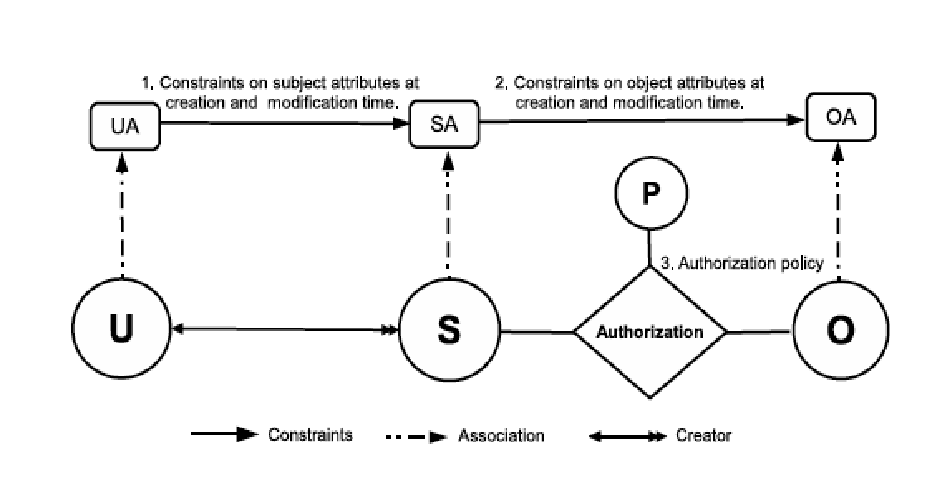
\includegraphics[width=0.3\textwidth]{eps/abac_model}
 \caption{Attribute Based Access Control Model.}
 \label{fig:abac}
\end{figure}

As shown in the diagram,   the authorization policy in this model (shown by the diamond in the figure) is specified with attributes from the subject/users and objects. Without giving any details, we would like to mention that the policy can include any number of user or object attributes.

The interested readers are encouraged to have a look at \cite{abac} where the model components and policy language are discussed in great detail. 

